\chapter{Abstraktion und Struktur}
\label{chap:V_abstraktion}


In den vorhergehenden Kapiteln wurde deutlich,
dass Naturgesetze\index{Naturgesetz}
nicht durch anschauliche Bilder,
sondern durch mathematische Beziehungen beschrieben werden.
Bewegung\index{Bewegung},
Wachstum\index{Wachstum}
und Dynamik\index{Dynamik}
lassen sich nur verstehen,
wenn Veränderung\index{Veränderung}
formal gefasst wird.
Damit stellt sich eine weiterführende Frage:
Wie ist es möglich,
dass abstrakte mathematische Begriffe
reale Naturphänomene so präzise erfassen?

Die Antwort liegt im Prinzip der Abstraktion\index{Abstraktion}.
Mathematik\index{Mathematik}
verzichtet bewusst auf viele Eigenschaften der Wirklichkeit,
um ihre strukturellen Merkmale freizulegen.
Sie beschreibt nicht,
\emph{was} ein Objekt stofflich ist,
sondern \emph{wie} es sich verhält
und in welchen Beziehungen es zu anderen Objekten steht.
Abstraktion ist daher kein Verlust an Realität\index{Realität},
sondern eine gezielte Reduktion auf das Wesentliche.

Struktur\index{Struktur}
bezeichnet genau das,
was unter dieser Reduktion erhalten bleibt.
Sie ist unabhängig vom konkreten Material,
vom Maßstab
oder vom Ort\index{Ort}.
Ob ein System aus Punkten,
Teilchen\index{Teilchen}
oder Feldern\index{Feld} besteht,
ist für die mathematische Struktur zunächst zweitrangig.
Entscheidend ist allein das Geflecht der Beziehungen,
das diese Elemente miteinander verbindet.

Dieses Kapitel untersucht,
wie Abstraktion und Struktur zusammenwirken
und warum sie für das Verständnis moderner Mathematik
und Physik\index{Physik} unverzichtbar sind.
Es zeigt,
dass Mathematik nicht deshalb erfolgreich ist,
weil sie die Wirklichkeit nachbildet,
sondern weil sie deren Strukturen freilegt.





% =====================================================
% 5.1 Vektoren und Räume
% =====================================================
\subsection{Vektoren und Räume}

Der Begriff des Vektors\index{Vektor}
gehört zu den bekanntesten Elementen der Mathematik\index{Mathematik}
und Physik\index{Physik}.
Im schulischen Zusammenhang erscheint er meist als Pfeil
mit Richtung, Länge und Orientierung.
Diese Vorstellung ist anschaulich und nützlich,
doch sie trifft nicht den eigentlichen Kern.
Ein Vektor ist nicht in erster Linie ein geometrisches Bild,
sondern ein abstraktes Element eines Raumes\index{Raum}.

Diese Verschiebung der Perspektive ist entscheidend.
Mathematik interessiert sich nicht dafür,
wie ein Vektor aussieht,
sondern dafür,
wie er sich zu anderen Vektoren verhält.
Addition\index{Addition},
Skalierung\index{Skalierung}
und Vergleich sind keine bloßen Rechenverfahren,
sondern Ausdruck einer zugrunde liegenden Struktur.
Erst durch solche Beziehungen wird ein Raum mathematisch bestimmt.

Ein Raum ist daher nicht einfach eine Menge von Punkten\index{Punkt}.
Er ist ein System von Relationen\index{Relation},
in dem bestimmte Operationen sinnvoll definiert sind.
Welche Objekte diesen Raum bilden,
ist zunächst zweitrangig.
Vektoren können Verschiebungen\index{Verschiebung} im Raum darstellen,
Geschwindigkeiten\index{Geschwindigkeit},
Kräfte\index{Kraft},
Zustände\index{Zustand}
oder abstrakte Informationsinhalte.
Entscheidend ist nicht ihre jeweilige Deutung,
sondern die Struktur\index{Struktur},
die sie gemeinsam besitzen.

Gerade hier zeigt sich die Kraft der Abstraktion\index{Abstraktion}.
Indem Mathematik von der konkreten Interpretation absieht,
werden sehr unterschiedliche Phänomene vergleichbar.
Ein und derselbe Vektorraum\index{Vektorraum}
kann Bewegungen beschreiben,
elektrische Felder\index{Feld} strukturieren
oder Zustände der Quantenmechanik\index{Quantenmechanik} repräsentieren.
Was sich ändert,
ist die physikalische Bedeutung --
nicht die mathematische Form.

Diese Sichtweise kehrt die gewohnte Denkweise um.
Nicht der Raum ist durch anschauliche Bilder festgelegt,
sondern die Elemente erhalten ihre Bedeutung
durch den Raum, in dem sie liegen.
Ein Vektor ist daher nicht \glqq an sich\grqq{} ein Pfeil,
sondern wird erst durch die Struktur des Raumes zu dem,
was er mathematisch ist.
Abstraktion bedeutet hier nicht Verzicht,
sondern Präzisierung.

Die Einführung von Vektorräumen markiert daher einen Wendepunkt.
Mathematik löst sich von anschaulichen Einzelformen
und formuliert Beziehungen,
die unabhängig von Dimension\index{Dimension},
Maßstab
oder physikalischem Kontext gültig sind.
Ein Raum kann endlich oder unendlich dimensional,
kontinuierlich oder diskret sein --
die formalen Beziehungen bleiben dieselben.

Damit wird verständlich,
warum die moderne Physik\index{Moderne Physik}
ohne solche abstrakten Räume nicht auskommt.
Felder sind keine bloßen Sammlungen von Zahlen,
sondern Elemente geeigneter Funktionsräume\index{Funktionsraum}.
Quantenzustände sind keine Bahnen,
sondern Vektoren in abstrakten Zustandsräumen\index{Zustandsraum}.
Die Wirklichkeit\index{Wirklichkeit}
wird damit nicht anschaulicher,
sondern relationaler beschrieben.

Vektoren und Räume sind deshalb kein technisches Hilfsmittel,
sondern ein grundlegendes Denkwerkzeug.
Sie zeigen exemplarisch,
wie Mathematik Wirklichkeit nicht einfach abbildet,
sondern ihre Ordnung strukturell erfasst.
Abstraktion ist hier nicht das Entfernen von Realität,
sondern die Bedingung dafür,
ihre Form überhaupt erkennen zu können.

Ein einfaches Beispiel macht diese Sichtweise anschaulich.
Betrachten wir einen zweidimensionalen Raum\index{zweidimensionaler Raum},
wie er aus der Ebene vertraut ist.
Ein Vektor wird dort häufig als Pfeil dargestellt,
der von einem Punkt zu einem anderen zeigt.
Entscheidend ist jedoch nicht seine konkrete Lage,
sondern seine Wirkung als Verschiebung.

Verschiebt man einen solchen Pfeil parallel,
ohne seine Richtung oder Länge zu verändern,
so bleibt er mathematisch derselbe Vektor.
Seine Bedeutung liegt nicht im Anfangspunkt,
sondern in der Beziehung zwischen Anfang und Ende.
Gerade diese Unabhängigkeit vom Ort\index{Ort}
kennzeichnet den abstrakten Vektorbegriff.

Besonders deutlich wird dies in der grafischen Darstellung:

\begin{center}
	\begin{tikzpicture}[scale=1.1]
		
		% Koordinatenachsen
		\draw[->] (-0.5,0) -- (4.5,0) node[right] {$x$};
		\draw[->] (0,-0.5) -- (0,3.5) node[above] {$y$};
		
		% Erster Vektor
		\draw[thick,->] (0.5,0.5) -- (2.5,1.5);
		
		% Zweiter (verschobener) Vektor
		\draw[thick,->] (1.0,2.0) -- (3.0,3.0);
		
	\end{tikzpicture}
\end{center}

Beide Pfeile stellen denselben Vektor dar,
obwohl sie an unterschiedlichen Orten eingezeichnet sind.
Für die Mathematik ist allein die Verschiebung relevant,
nicht ihre Einbettung in einen bestimmten Punkt der Ebene.
Der Raum liefert den Rahmen,
in dem solche Relationen sinnvoll definiert sind.

Dieses einfache Beispiel zeigt den Kern der Abstraktion:
Die geometrische Zeichnung dient nur der Veranschaulichung.
Der eigentliche Gegenstand der Mathematik
ist die Struktur,
die allen möglichen Darstellungen gemeinsam ist.
Vektoren sind nicht Pfeile im Raum --
sie sind Elemente eines Raumes,
der durch seine Beziehungen definiert ist.
% =====================================================
% 5.2 Symmetrien und Invarianz
% =====================================================

\subsection{Symmetrien und Invarianz}

Nachdem Vektoren\index{Vektor}
als Elemente abstrakter Räume\index{Raum} eingeführt wurden,
stellt sich eine weiterführende Frage:
Woran erkennt man die Struktur\index{Struktur} eines solchen Raumes?
Die Antwort liegt nicht in einzelnen Objekten,
sondern in dem,
was sich bei Veränderungen\index{Veränderung} \emph{nicht} ändert.
Genau hier setzt der Begriff der Symmetrie\index{Symmetrie} an.

Im alltäglichen Sprachgebrauch
wird Symmetrie oft mit Spiegelbildern
oder ästhetischer Ausgewogenheit verbunden.
In der Mathematik\index{Mathematik}
und Physik\index{Physik}
hat der Begriff jedoch eine präzisere Bedeutung.
Eine Symmetrie liegt vor,
wenn ein Objekt oder ein System
unter einer bestimmten Veränderung unverändert bleibt.
Entscheidend ist dabei nicht die Veränderung selbst,
sondern das,
was invariant\index{Invarianz} bleibt.

Diese Idee lässt sich leicht verallgemeinern.
Eine Verschiebung\index{Verschiebung} im Raum
ändert die Lage eines Körpers,
aber nicht seine Form.
Eine Drehung\index{Drehung}
verändert die Orientierung,
aber nicht die Abstände zwischen Punkten\index{Punkt}.
In beiden Fällen bleiben bestimmte Eigenschaften erhalten.
Gerade diese Erhaltungseigenschaften
offenbaren die zugrunde liegende Struktur.

In der Physik spielen solche Invarianzen eine zentrale Rolle.
Naturgesetze\index{Naturgesetz}
zeichnen sich dadurch aus,
dass sie unabhängig von Ort\index{Ort},
Zeit\index{Zeit}
oder Orientierung gelten.
Ob ein Experiment hier oder dort durchgeführt wird,
ob es heute oder morgen stattfindet,
ob das Koordinatensystem\index{Koordinatensystem} gedreht wird --
das Gesetz bleibt dasselbe.
Diese Unabhängigkeit ist kein Zufall,
sondern Ausdruck einer tiefen Symmetrie der Natur.

\begin{DidacticBox}[Was Symmetrie bedeutet]
	\phantomsection\label{box:symmetrie}
	Symmetrie beschreibt nicht Gleichförmigkeit,
	sondern Erhaltung.
	Ein System ist symmetrisch,
	wenn bestimmte Eigenschaften unter Veränderungen unverändert bleiben.
	
	Nicht die Veränderung ist entscheidend,
	sondern das,
	was sich \emph{nicht} verändert.
\end{DidacticBox}

Mathematisch wird diese Idee
durch Transformationen\index{Transformation} präzisiert.
Eine Transformation ist eine erlaubte Veränderung eines Systems --
etwa eine Verschiebung,
Drehung
oder Spiegelung\index{Spiegelung}.
Bleibt eine bestimmte Eigenschaft unter dieser Transformation erhalten,
so spricht man von Invarianz.
Symmetrien sind damit keine geometrischen Spielereien,
sondern Aussagen über strukturelle Stabilität\index{Stabilität}.

Diese Sichtweise ist grundlegend
für das Verständnis moderner Physik\index{Moderne Physik}.
Erhaltungsgrößen\index{Erhaltungsgröße}
wie Energie\index{Energie},
Impuls\index{Impuls}
oder Drehimpuls\index{Drehimpuls}
sind keine isolierten Postulate,
sondern Konsequenzen von Symmetrien.
Sie entstehen nicht aus Einzelmessungen,
sondern aus der Struktur der zugrunde liegenden Gesetze.
Die Mathematik macht diese Zusammenhänge sichtbar,
noch bevor ein konkretes Experiment betrachtet wird.

Bemerkenswert ist,
dass Symmetrien unabhängig
vom jeweiligen Trägermaterial sind.
Sie gelten für Teilchen\index{Teilchen},
Felder\index{Feld}
oder abstrakte Zustandsräume\index{Zustandsraum} gleichermaßen.
Was sich ändert,
ist die Interpretation --
nicht die Struktur.
Symmetrie ist damit
ein universelles Organisationsprinzip\index{Ordnungsprinzip},
das weit über anschauliche Geometrie hinausreicht.

In dieser Perspektive wird deutlich,
warum Abstraktion\index{Abstraktion} notwendig ist.
Erst der Verzicht auf konkrete Bilder
macht es möglich,
die invarianten Eigenschaften eines Systems freizulegen.
Mathematik beschreibt nicht,
wie ein System aussieht,
sondern welche Veränderungen es zulässt,
ohne sein Wesen zu verlieren.

Symmetrien und Invarianz
bilden deshalb einen zentralen Baustein moderner Naturbeschreibung.
Sie verbinden abstrakte Räume
mit physikalischer Realität\index{Realität}
und zeigen,
dass die Ordnung der Natur
weniger in ihren Erscheinungen
als in den Beziehungen\index{Relation} liegt,
die diese Erscheinungen miteinander verknüpfen.

Ein einfaches Beispiel verdeutlicht
den Zusammenhang zwischen Symmetrie und Invarianz.
Betrachten wir ein physikalisches System,
das sich entlang einer Geraden bewegt.
Verschieben wir das gesamte System
um eine feste Strecke,
so ändern sich die beteiligten Orte,
nicht jedoch das zugrunde liegende Bewegungsgesetz\index{Bewegungsgesetz}.

Für die Physik ist entscheidend,
dass das Gesetz unabhängig vom gewählten Bezugspunkt\index{Bezugssystem} gilt.
Ob die Bewegung an einem Ort beginnt
oder an einem anderen,
spielt keine Rolle.
Die Verschiebung verändert die Beschreibung,
aber nicht die Struktur des Gesetzes.
Genau diese Unabhängigkeit
bezeichnet man als Translationsinvarianz\index{Translationsinvarianz}.

Beide Darstellungen beschreiben somit dasselbe physikalische Gesetz,
obwohl die Systeme an unterschiedlichen Orten liegen.
Die Verschiebung verändert die Koordinaten\index{Koordinate},
nicht jedoch die Beziehungen zwischen den beteiligten Größen.
Das Gesetz bleibt invariant unter Translation\index{Translation}.

\begin{center}
	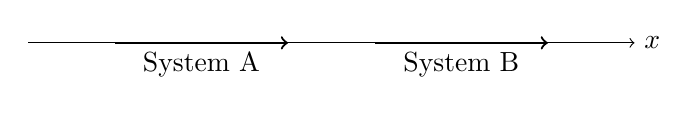
\begin{tikzpicture}[scale=1.1]
		
		% Achse
		\draw[->] (-0.5,0) -- (6.5,0) node[right] {$x$};
		
		% erstes System
		\draw[thick,->] (0.5,0) -- (2.5,0);
		\node[below] at (1.5,0) {System A};
		
		% zweites (verschobenes) System
		\draw[thick,->] (3.5,0) -- (5.5,0);
		\node[below] at (4.5,0) {System B};
		
	\end{tikzpicture}
\end{center}

Dieses Beispiel zeigt den Kern der Symmetrieidee:
Ein Naturgesetz ist genau dann fundamental,
wenn es unabhängig von willkürlichen Festlegungen
wie Ort,
Zeit
oder Orientierung gilt.
Symmetrien sind daher keine Zusatzannahmen,
sondern ein Prüfstein
für die Allgemeingültigkeit physikalischer Gesetze.


% =====================================================
% 5.3 Mathematik als universelles Strukturprinzip
% =====================================================
\subsection{Mathematik als universelles Strukturprinzip}

Die bisherigen Überlegungen zeigen,
dass Mathematik\index{Mathematik}
nicht mit einzelnen Dingen,
sondern mit Strukturen\index{Struktur} arbeitet.
Gerade deshalb kann dieselbe mathematische Form
in sehr unterschiedlichen Bereichen der Natur\index{Natur}
wiederkehren.

Was in der Mechanik\index{Mechanik}
als Bewegungsgesetz erscheint,
kann in der Elektrodynamik\index{Elektrodynamik},
in der Quantenphysik\index{Quantenphysik}
oder in der Feldtheorie\index{Feldtheorie}
in neuer Gestalt wieder auftreten.
Die beschriebenen Objekte unterscheiden sich,
doch die zugrunde liegenden Beziehungen bleiben vergleichbar.
Unterschiedlich sind die Bedeutungen,
nicht die Form.

Darin liegt die Universalität der Mathematik\index{Universalität}.
Sie beschreibt nicht die stoffliche Beschaffenheit der Dinge,
sondern die Muster,
die verschiedenen Systemen gemeinsam sind.
Wenn unterschiedliche Phänomene
denselben strukturellen Gesetzen folgen,
erscheinen sie notwendig in derselben mathematischen Sprache.

Diese Universalität ist kein Zufall
und keine bloße Folge menschlicher Vereinbarung.
Sie ergibt sich aus der Art,
wie Mathematik arbeitet:
durch Abstraktion,
durch Relationen
und durch die Freilegung invarianten Zusammenhangs.
Gerade deshalb kann sie
über einzelne Bereiche hinausreichen
und zum allgemeinen Strukturprinzip der Naturbeschreibung werden.

Mathematik ist damit nicht nur ein Werkzeug,
mit dem man bekannte Phänomene ordnet.
Sie zeigt auch,
welche Formen überhaupt als allgemeingültige Beschreibung in Frage kommen.
Was strukturell instabil oder mathematisch inkonsistent ist,
kann keinen fundamentalen Anspruch erheben.

Damit wird verständlich,
warum Mathematik in so unterschiedlichen Bereichen
dieselbe Sprache spricht:
nicht weil die Phänomene gleich wären,
sondern weil ihre Struktur verwandt ist.
Gerade in dieser strukturellen Verwandtschaft
liegt ihre Universalität.



% =====================================================
% 5.4 Abstraktion als Weg zur Wirklichkeit
% =====================================================

\subsection{Abstraktion als Weg zur Wirklichkeit}

Im alltäglichen Sprachgebrauch
gilt Abstraktion\index{Abstraktion}
oft als Gegensatz zur Wirklichkeit\index{Wirklichkeit}.
Was abstrakt ist,
erscheint fern,
theoretisch
oder künstlich.
In der Mathematik\index{Mathematik}
und Physik\index{Physik}
bedeutet Abstraktion jedoch etwas grundlegend anderes.
Sie ist kein Entfernen von Realität,
sondern ein gezieltes Herausfiltern dessen,
was für das Verständnis wesentlich ist.

Schon einfache physikalische Modelle\index{Modell}
arbeiten abstrakt.
Ein Körper wird als Punkt\index{Punkt} behandelt,
Reibung\index{Reibung} wird vernachlässigt,
ideale Bedingungen\index{Idealisierung} werden angenommen.
Solche Vereinfachungen sind keine Täuschungen,
sondern bewusste Entscheidungen.
Sie machen Strukturen\index{Struktur} sichtbar,
die in der Komplexität realer Situationen
sonst verborgen blieben.

Abstraktion wirkt dabei wie ein Vergrößerungsglas.
Indem Nebeneffekte ausgeblendet werden,
treten die grundlegenden Beziehungen\index{Relation} deutlicher hervor.
Ein Modell ist nicht deshalb nützlich,
weil es alles enthält,
sondern weil es genau das Richtige weglässt.
Die Wirklichkeit wird nicht kopiert,
sondern in ihrer Ordnung freigelegt.

\begin{DidacticBox}[Abstraktion und Realität]
	\phantomsection\label{box:abstraktion}
	Abstraktion bedeutet nicht Realitätsverlust.
	Sie bedeutet Fokussierung.
	
	Was weggelassen wird,
	sind kontextabhängige Eigenschaften.
	Was erhalten bleibt,
	ist die zugrunde liegende Struktur.
\end{DidacticBox}

Gerade die moderne Physik\index{Moderne Physik}
zeigt die Notwendigkeit dieses Vorgehens.
Quantenmechanik\index{Quantenmechanik},
Relativitätstheorie\index{Relativitätstheorie}
und Feldtheorien\index{Feldtheorie}
operieren mit Begriffen,
die sich jeder unmittelbaren Anschauung entziehen.
Dennoch liefern sie die präzisesten Vorhersagen\index{Vorhersage},
die die Physik kennt.
Ihre Nähe zur Wirklichkeit
zeigt sich nicht in Bildern,
sondern in der Genauigkeit ihrer Aussagen.

Diese Entwicklung ist kein Zufall.
Je tiefer man in die Struktur der Natur\index{Natur} eindringt,
desto weniger tragen anschauliche Vorstellungen.
Abstrakte Begriffe ersetzen konkrete Bilder,
weil sie unter verschiedenen Darstellungen invariant\index{Invarianz} bleiben.
Die Mathematik macht genau diese invarianten Strukturen sichtbar
und löst sie von subjektiver Wahrnehmung\index{Wahrnehmung}.

Abstraktion ist damit kein Umweg,
sondern der direkte Weg zur Wirklichkeit.
Sie ermöglicht es,
allgemeine Gesetzmäßigkeiten\index{Naturgesetz} zu erkennen,
die über einzelne Beobachtungen hinausgehen.
Was zunächst fern erscheint,
erweist sich bei genauerem Hinsehen
als das Verlässlichste,
was wir über die Natur aussagen können.

In diesem Sinn bildet Abstraktion
den Abschluss und zugleich den Übergang dieses Kapitels.
Sie verbindet die mathematische Sprache der Natur
mit ihrer strukturellen Ordnung
und öffnet den Blick auf jene Bereiche,
in denen Struktur nicht nur in deterministischen Gesetzen,
sondern auch in Wahrscheinlichkeit\index{Wahrscheinlichkeit},
Zufall\index{Zufall}
und Unsicherheit\index{Unsicherheit} sichtbar wird.
Auch dort bleibt Mathematik
kein Gegenpol zur Wirklichkeit,
sondern ihr präzisestes Ausdrucksmittel.

\subsection*{Übergang: Struktur und Zufall}

Die bisherigen Überlegungen haben gezeigt,
dass Mathematik ihre Stärke gerade dort entfaltet,
wo sie von der Oberfläche der Erscheinungen absieht
und die zugrunde liegende Struktur freilegt.
Doch damit stellt sich eine neue, schwierigere Frage:
Was geschieht,
wenn uns die Welt nicht geordnet,
sondern zufällig erscheint?

Nicht alle Phänomene folgen einfachen,
deterministischen Bahnen.
Würfe, Zerfälle, Schwankungen und unvorhersehbare Ereignisse
scheinen sich dem Anspruch strenger Gesetzmäßigkeit zu entziehen.
Gerade hier entscheidet sich,
wie weit die mathematische Beschreibung tatsächlich reicht.
Ist Zufall ein Merkmal der Welt selbst --
oder nur ein Zeichen dafür,
dass unsere Beschreibung an Grenzen stößt?

Damit führt die Frage nach Abstraktion und Struktur
direkt zum nächsten Problem:
zur Rolle des Zufalls,
der Wahrscheinlichkeit
und der Unsicherheit in unserem Verständnis der Wirklichkeit.